\documentclass{beamer}
\input{../flat-blue-theme.inc}

\usepackage[utf8]{inputenc}
\usepackage[OT1]{fontenc}
\usepackage[ngerman]{babel}
\usepackage{lastpage}
\usepackage{tikz}
\usepackage{tabularx}
\usepackage{hyperref}
\usepackage{xifthen}
\usepackage{multicol}

\usepackage{tikz}
\usetikzlibrary{positioning}
\usetikzlibrary{arrows}

\usepackage{lmodern}
%\usepackage{libertine}

\renewcommand\footnoterule
{
	% Original implementation just with gray color
	\color{gray}
	\kern-3pt 
	\hrule width 2in 
	\kern 2.6pt
}
\renewcommand\thefootnote{\tiny\textcolor{gray}{\arabic{footnote}}}
\let\oldfootnote\footnote
\renewcommand{\footnote}[1]
{%
	\oldfootnote
	{
		\tiny
		\textcolor{gray}{#1}
	}%
}
\newcommand{\citewiki}[2][]
{%
	\footnote
	{
		\ifthenelse{\isempty{#1}}
		{
			Quelle: \href{https://de.wikipedia.org/wiki/#2}{Wikipedia:#2}
		}
		{
			Quelle: \href{https://de.wikipedia.org/wiki/#2}{Wikipedia:#1}
		}
	}
}
\newcommand{\citeurl}[2]
{
	\footnote
	{
		\tiny
		\textcolor{gray}
		{
			Quelle: \href{#1}{#2}
		}
	}
}
\newcommand{\money}[2][green!45!gray]{
	\node
	[
		fill=#1,
		minimum height=0.4cm,
		minimum width=0.9cm,
		inner sep=0pt,
		rounded corners=0.1cm,
		draw=#1!80!black,
		thick
	] at #2 {\scriptsize\color{white}€};
}
\newcommand{\moneyLight}[1]{
	\money[green!33!lightgray!75!white]{#1}
}
\newcommand{\smallmoney}[2][green!45!gray]{
	\node
	[
		fill=#1,
		minimum height=0.3cm,
		minimum width=0.675cm,
		inner sep=0pt,
		rounded corners=0.075cm,
		draw=green!50!black,
		semithick
	] at #2 {\tiny\color{white}€};
}

\newcommand{\wkn}[1]{\href{https://www.finanzen.net/anleihen/#1}{#1}}

\setbeamercovered{invisible}

\author[Hauke Stieler]{Hauke Stieler\\\href{mailto:4stieler@informatik.uni-hamburg.de}{4stieler@inf}}
\title{Stonks}
\date{\today}

\begin{document}
	{
		\setbeamertemplate{headline}{}
		\setbeamertemplate{background}{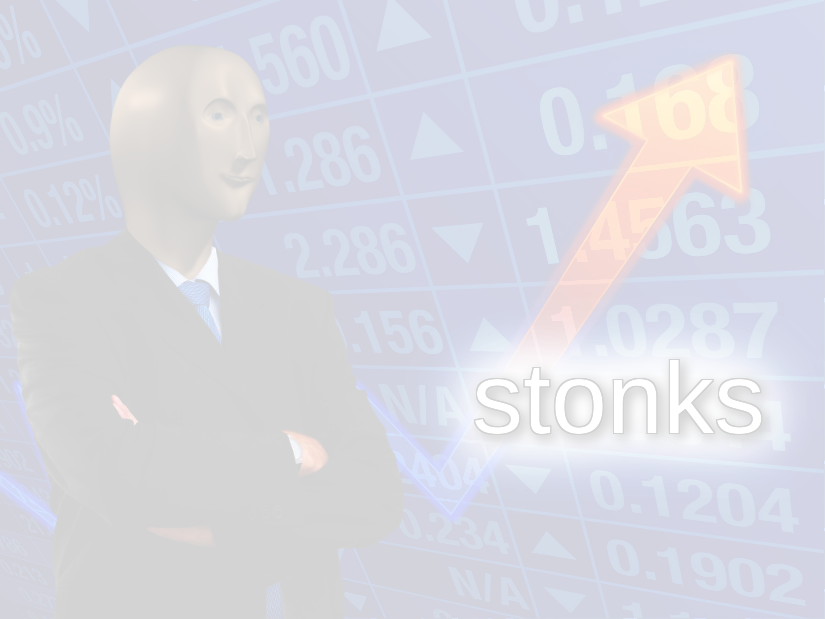
\includegraphics[width=\paperwidth,trim=0 0 0 3.5cm]{images/stonks-title-full}}
		\maketitle
	}
	
	\begin{frame}{Disclaimer}
		\begin{center}
			Diese Präsentation inklusive Vortrag ist keine Rechts-, Steuer-, Anlage- oder Finanzberatung!\n
			Der Handel mit Finanzprodukten ist mit Risiken behaftet und kann zum TOTALVERLUST des eingesetzten Kapitals führen.\n
			Es besteht keinerlei Garantie für die Richtigkeit der Informationen in dieser Präsentation.\n
			Alle genannten Finanzprodukte dienen nur als anschauliche Beispiele und stellen keinerlei Empfehlung dar.
		\end{center}
	\end{frame}

	\begin{frame}
		\begin{center}
			Was für Vorwissen hast du?
		\end{center}
	\end{frame}

	\begin{frame}
		\tableofcontents[hidesubsections]
	\end{frame}
	
	\section{Basics}
	
		\begin{frame}
			\tableofcontents[currentsection,hideallsubsections]
		\end{frame}
	
		\subsection{Begrifflichkeiten}
		
		\begin{frame}
			\begin{description}[labelwidth=0cm]
				\item[Gewinn/Verlust] Differenz Kauf- \& Verkaufspreis\pause
				\item[Kurs] Aktueller Preis einer Aktie an einer bestimmten Börse\pause
				\item[Rendite] Gewinn relativ zum Einsatz (in Prozent)\pause
				\item[Kapital] = Mittel = Geld (meistens)\pause
				\item[Anleger] Auch \textit{Investor}, nimmt am Finanzmarkt teil, z.B. durch Investitionen\pause
				\item[Risiko] Wahrscheinlichkeit des Eintretens eines negativen Ereignisses\pause
				\item[Portfolio] Sammlung an Wertpapieren
				\item[Wertpapier] Z.B. Aktien, Anleihen, ETFs, ...
			\end{description}
		\end{frame}
		
		\subsection{Investieren (Geld anlegen)}
		
			\begin{frame}
				\begin{definition}
					Einsatz von Kapital für einen bestimmten Verwendungszweck.\citewiki{Investition}
				\end{definition}
				\begin{itemize}
					\item Motivation: Glaube an die Qualität des Unternehmens
					\item Horizont: Langfristig (Jahre/Jahrzehnte)
				\end{itemize}\n
				\textbf{Beispiele:}
				\begin{itemize}
					\item Kauf von Aktien zum Vermögensaufbau.
					\item Kauf eines Buches zum lernen für eine Uni-Veranstaltung.
					\item Sport treiben zum Erhalt der körperlichen Gesundheit.
				\end{itemize}
			\end{frame}
		
		\subsection{Spekulieren (Trading)}
		
			\begin{frame}
				\begin{definition}
					Risikoreiches Ausnutzen von Preisschwankungen zur Gewinnmitnahme.\citewiki{Spekulation\_(Wirtschaft)}
				\end{definition}
				\begin{itemize}
					\item Motivation: Externe Faktoren zur Gewinnerzeugung nutzen
					\begin{itemize}
						\item Böse formuliert: Sich an Fehlentscheidungen/""Hoffnungen/Unwissen/... anderer bereichern
					\end{itemize}
					\item Horizont: Kurzfristig (Sekunden bis Monate)
				\end{itemize}\n
				\textbf{Beispiele:}
				\begin{itemize}
					\item Kauf (irgend)einer Aktie, Verkauf am Folgetag.
					\item Bunkern von Getreide in Hoffnung auf Kriege und Wirtschaftskrisen.
				\end{itemize}
			\end{frame}
		
		\subsection{Sparen}
		
			\begin{frame}
				\begin{definition}
					Verzicht auf Verbrauch von Kapital zur späteren Verwendung.\citewiki{Sparen}
				\end{definition}\hfill
				
				\textbf{Beispiele:}
				\begin{itemize}
					\item Monatlich 300€ nicht ausgeben
					\item Einmalig 10.000€ auf ein Festgeldkonto
					\item Bis zum 18. Geburtstag des Kindes jährlich 500€ kontinuierlich investieren
				\end{itemize}
			\end{frame}
		
		\subsection{Zins und Zinseszins}
		
			\begin{frame}{Begrifflichkeiten}
				\begin{description}[labelwidth=0cm]
					\item[Gläubiger] Kredit\textit{geber}, vergibt Kredite (z.B. Bank)\pause
					\item[Schuldner] Kredit\textit{nehmer}, empfängt den Kredit (z.B. Du)
				\end{description}
			\end{frame}
		
			\begin{frame}{Zinsen}
				\begin{definition}
					Zinsen sind das Entgeld für zeitweise überlassenes Kapital (z.B. ein Kredit) vom Schuldner zum Gläubiger.\citewiki{Zins}
				\end{definition}
				\textbf{Beispiele:}
				\begin{multicols}{2}
					\begin{itemize}
						\item Sparbuch:\\
						\begin{tikzpicture}[->,>=stealth']
							\node (i) at (0,0) {Du};
							\node (b) at (3,0) {Bank};
							
							\draw (i) to [bend left=10] node[above,font=\tiny] {Sparbetrag} (b);
							\draw (b) to [bend left=10] node[below,align=center,font=\tiny] {Sparbetrag\\+ Zinsen} (i);
						\end{tikzpicture}
						\columnbreak
						\item Kredit:\\
						\begin{tikzpicture}[->,>=stealth']
							\node (b) at (0,0) {Bank};
							\node (i) at (3,0) {Du};
							
							\draw (b) to [bend left=10] node[above,font=\tiny] {Kredit} (i);
							\draw (i) to [bend left=10] node[below,align=center,font=\tiny] {Kredit\\+ Zinsen} (b);
						\end{tikzpicture}
					\end{itemize}
				\end{multicols}
				\vspace{-0.25cm}
				{\tiny Reale Welt sieht anders aus, Stichwort \href{https://de.wikipedia.org/wiki/Leitzins}{Leitzins} und \href{https://de.wikipedia.org/wiki/Buchgeld}{Giralgeld}.}
			\end{frame}
		
			\begin{frame}{Zinsen}
				\begin{itemize}
					\item Höhe der Zinsen hängt ab von:
					\begin{itemize}
						\item Leitzins
						\item Bonität des Schuldners
						\item Allgemeiner wirtschaftlicher Lage
					\end{itemize}
					\item Daumenregel beim Investieren
					\begin{itemize}
						\item Hohe Zinsen \textrightarrow\ hohes Risiko!
						\item Zinsen $\approx$ Schmerzensgeld / Belohnung für eingegangenes Risiko
					\end{itemize}
				\end{itemize}
			\end{frame}
		
			\begin{frame}{Zinsen: Der Zinseszins-Effekt}
				\begin{definition}
					Zinsen, die auf Kapital mit zuvor hinzugefügten Zinsen gezahlt werden.\citewiki{Zinseszins}
				\end{definition}
				\textbf{Einfach gesagt:}\\
				Zinsen auf Zinsen \textrightarrow\ exponentielles Wachstum\n
				
				\textbf{Beispiel Sparbuch} mit 10\% Zinsen:
				\begin{itemize}
					\item 2021: 100,00€ \textrightarrow\ 10,00€ Zinsen \textrightarrow\ 110,00€ am Jahresende
					\item 2022: 110,00€ \textrightarrow\ 11,00€ Zinsen \textrightarrow\ 121,00€
					\item 2023: 121,00€ \textrightarrow\ 12,\textbf{10}€ Zinsen \textrightarrow\ 133,10€
				\end{itemize}
			\end{frame}
	
	\section{Finanzprodukte}
	
		\begin{frame}
			\tableofcontents[currentsection,hideallsubsections]
		\end{frame}
	
		\begin{frame}{Begrifflichkeiten}
			\begin{description}[labelwidth=0cm]
				\item[Wertpapier] Urkunde, die Rechte gegenüber einem Schuldner verbrieft\citewiki{Wertpapier}(Beispiel: Aktie)
				\item[Volatilität] Größe der Schwankungen im Kursverlauf eines Wertpapiers\citewiki[Volatilität]{Volatilit\%C3\%A4t}(aka Varianz/""Standardabweichung)
				\item[WKN] \textbf{W}ertpapier\textbf{k}enn\textbf{n}ummer (z.B. A1R1BN)
				\item[ISIN] \textbf{I}nternational \textbf{S}ecurities \textbf{I}dentification \textbf{N}umber (z.B. XS0913868369)
			\end{description}
		\end{frame}
	
		\subsection{Aktien}
		
			\begin{frame}
				\vspace{0.5cm}
				\begin{center}
					Was ist eine Aktie?
				\end{center}
			\end{frame}
			
			\begin{frame}
				\begin{itemize}
					\item Erste Aktie 1288\citewiki{Aktie}
					\item Verbrieft einen Anteil an Unternehmen
					\begin{itemize}
						\item Mitbesitzer des Unternehmens \textrightarrow\ Aktionär
					\end{itemize}
					\item Rechte
					\begin{itemize}
						\item Stimmrecht
						\item Dividendenanspruch
					\end{itemize}
					\item Pflichten
					\begin{itemize}
						\item Aktie bezahlen (Einlage in Grundkapital)
						\item Treuepflicht: Im Interesse des Unternehmens \& anderer Anleger handeln
					\end{itemize}
					\item Jährliche Hauptversammlung besuchen
				\end{itemize}
			\end{frame}
		
			\begin{frame}{Dividende}
				\begin{definition}
					Auszahlung eines Teils des Gewinns an die Aktionäre.\citewiki{Dividende}
				\end{definition}
				\hfill\\
				\begin{itemize}
					\item Optional (s. "`Alphabet Inc."' aka Google)
					\item Höhe wird von Aktionären auf Hauptversammlung bestimmt
					\item Dividenden sind eine Art der Ausschüttung von \textbf{Gewinnen}
				\end{itemize}
			\end{frame}
				
			\begin{frame}{Dividende (Beispiel)}
				Beispiel BASF:\citeurl{https://www.finanzen.net/bilanz_guv/basf}{finanzen.net}\\
				\hfill\\
				\begin{tabularx}{\linewidth}{l|X|X|X|X}
					Daten & 2018 & 2019 & 2020 & 2021\\
					\hline\hline
					Gewinn (mio. €)		& 4.707 & 2.737 & -1.418 & 5.523 \\
					Dividende (mio. €) \footnote{An Aktionäre, weitere Dividenden ggf. an anderen Gesellschafter}
										& 2.847 & 2.939 &  3.031 & 3.031 \\
					Dividende pro Aktie	& 3,20  & 3,30  &  3,30  & 3,40  
					\uncover<2->{\\Dividendenrendite	& 5,3\% & 4,9\% &  5,1\% & 5,5\%}
				\end{tabularx}\\
				\hfill\\
				\hfill\\
				\uncover<2->{
					Dividendenrendite = $\frac{\text{Dividende}}{\text{Aktienkurs}}$\\
					{\tiny (Wie viel Dividende bekäme ich für $x$ € an Investition?)}
				}
\			\end{frame}
		
		\subsection{Anleihen}
		
			\begin{frame}
				\begin{definition}
					Verzinsliches Wertpapier mit Recht auf Rückzahlung und Zinsen.\citewiki{Anleihe}
				\end{definition}
				Name ist Programm: An\textbf{leihe} \textrightarrow\ Rückzahlung + Zinsen
				\begin{itemize}
					\item Auch: Rentenpapier, Schuldverschreibung, Bond
					\item Feste Laufzeit
					\item Zinssatz (fest oder variabel), jährlich gezahlt
					\item Ggf. handelbar
					\item Staatsanleihen/Unternehmensanleihen
				\end{itemize}
			\end{frame}
		
			\begin{frame}{Beispiel (BASF)}
				Anleihen \href{https://www.finanzen.net/anleihen/a1r1bn-basf-se-anleihe}{A1R1BN} und \href{https://www.finanzen.net/anleihen/a11qc7-basf-se-anleihe}{A11QC7}:
				\begin{center}
					\begin{tabularx}{8cm}{l|l|l|l}
						WKN				& Von			& Bis					& Zins		\\
						\hline
						\wkn{A1R1BN}	& 04.02.2014	& 03.02.20\textbf{21}	& 1,875\%	\\
						\wkn{A11QC7}	& 12.02.2014	& 11.02.20\textbf{43}	& 3,250\%	\\
					\end{tabularx}
				\end{center}
			\end{frame}
		
		\subsection{Exkurs: Geschäftsanteil}
		
			\begin{frame}
				\begin{definition}
					Teil einer GmbH / Genossenschaft, der von einem Gesellschafter erworben werden kann.\citewiki{Geschäftsanteil}
				\end{definition}
			
				\begin{itemize}
					\item Beitrag zum Stammkapital (GmbH) oder Geschäftsguthabens (Genossenschaft)
					\item Dividende/Ausschüttung (z.B. GLS: 1-3\%)
					\item In der Regel: Kunde / Mitarbeiter sein
				\end{itemize}
			\end{frame}
		
		\subsection{Index}
		
			\begin{frame}
				\begin{definition}
					Kennzahl zur repräsentativen Dokumentation eines Teilmarktes.\citewiki{Aktienindex}
				\end{definition}
			
				\begin{itemize}
					\item Abstraktion auf Punktesystem
					\item Zeitliche Entwicklung spiegelt hypothetisches Portfolio wieder
					\item Kursindex:
					\begin{itemize}
						\item Aktienkurs bestimmt Index
						\item Dividenden werden ignoriert
						\item Beispiele: Dow Jones, FTSE 100, S\&P 500, Euro Stoxx 50
					\end{itemize}
					\item Performanceindex:
					\begin{itemize}
						\item Aktienkurs + Dividenden bestimmen Index
						\item Beispiel: DAX
					\end{itemize}
				\end{itemize}
			\end{frame}
		
			\begin{frame}{Beispiel (DAX)}
				\begin{itemize}
					\item DAX = \textbf{D}eutscher \textbf{A}ktieninde\textbf{x}\citewiki{DAX}
					\item Quasi TOP 40 der deutschen Unternehmen
					\item Geschwister: MDAX, SDAX, TecDAX, DivDAX, ...
					\item Aufnahmekriterium \& Gewichtung: Streubesitz-Marktkapitalisierung
					\item Maximales Gewicht: 10\%
					\item Simple Formel:\pause
					\[
						\text{I}_t = K_T \cdot B \cdot \frac
						{
							\sum_{i=1}^{n} p_{it} \cdot q_{iT} \cdot ff_{iT} \cdot c_{it}
						}
						{
							\sum_{i=1}^{n} p_{i0} \cdot q_{i0}
						}\hspace{1cm}
					\]
				\end{itemize}
			\end{frame}
		
		\subsection{Fonds}
		
			\begin{frame}
				\begin{definition}
					Verwaltetes Sondervermögen, welches in festgelegte Finanzprodukte investiert wird.\citewiki{Investmentfonds}
				\end{definition}\hfill
			
				\textbf{Einfacher gesagt:}\\
				Sammlung an Aktien, Anleihen, etc. in die man investieren kann.
			\end{frame}
		
			\begin{frame}
				\begin{itemize}
					\item Kategorien: Länder, Branchen, Unternehmensgröße\pause
					\item Aktiv
					\begin{itemize}
						\item Fondmanager beobachtet und analysiert Markt
						\item Ziel: Besser sein als "`der Markt"'
						\item Ziel erreichen nur sehr wenige
						\item Hohe Kosten (TER): ca. 1,3-2,5\%\footnote{z.B. \href{https://www.comdirect.de/inf/fonds/LU0552028770}{Amundi Funds Emerging Markets Equity Focus (ISIN: LU0552028770)}}
					\end{itemize}\pause
					\item Passiv\pause
					\begin{itemize}
						\item Keine Anpassungen durch Fondmanager
						\item Meist Abbildung eines Index (s. \nameref{subsec:etfs})
						\item Niedrige Kosten (ca. 0,02\footnote{z.B. \href{https://de.extraetf.com/etf-profile/LU1781541096}{Lyxor Core Morningstar UK UCITS (ISIN: LU1781541096)}}-0,87\%\footnote{z.B. \href{https://de.extraetf.com/etf-profile/IE00BYPLS672}{L\&G Cyber Security UCITS (ISIN: IE00BYPLS672)}})
					\end{itemize}\pause
					\item Kein direkter Besitz der Aktien!
				\end{itemize}
			\end{frame}
		
			\begin{frame}
				\hspace*{-0.75cm}
				\begin{tikzpicture}[->,>=stealth']
					\node (s) at (0,0) {
\includegraphics[width=1.25cm,trim=0 0 0 -1.35cm]{images/stonks-guy}};
					
					\node (i) at (3.5,0) {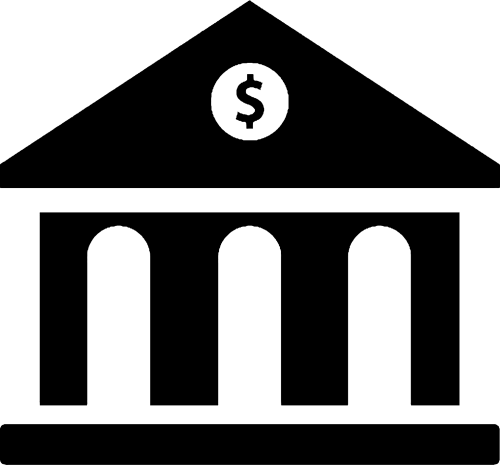
\includegraphics[width=1.25cm]{images/bank}};
					\node[below=0cm of i,align=center] {\small Investment-\\gesellschaft};
					
					\node (b) at (7,0) {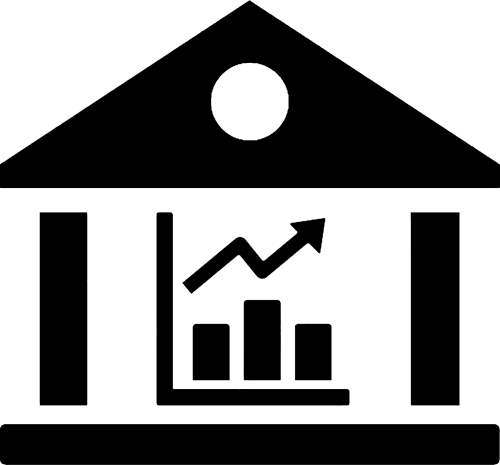
\includegraphics[width=1.25cm]{images/stockmarket}};
					\node[below of=b] {\small Börse};
					
					\node[xscale=-1] (s2) at (10.5,0) {
\includegraphics[width=1.25cm,trim=0 0 0 -1.35cm]{images/stonks-guy}};
					
					\onslide<2>
					{
						\money{(1.5,1)}
						\money{(1.6,0.9)}
						\money{(1.7,0.8)}
						\draw[thick] (s) to [bend left=10] (i);
					}
				
					\onslide<3-5>
					{
						\moneyLight{(3.5,1)}
						\draw[thick,gray!50!white] (s) to [bend left=10] (i);
					}
				
					\onslide<3>
					{
						\money{(5.25,1)}
						\money{(5.35,0.9)}
						\draw[thick] (i) to [bend left=10] (b);
					}
				
					\onslide<4->
					{
						\moneyLight{(7,1)}
						\draw[thick,gray!50!white] (i) to [bend left=10] (b);
					}
				
					\onslide<4>
					{
						\money{(8.75,1)}
						\draw[thick] (b) to [bend left=10] (s2);
						\draw[thick] (s2) to [bend left=10] (b);
						\node at (8.75,-1) {
\includegraphics[width=0.75cm]{images/stock}};
					}
					
					\onslide<5>
					{
						\draw[thick] (b) to [bend left=10] (i);
						\node at (5.4,-1) {
\includegraphics[width=0.75cm]{images/stock}};
						\node at (5.55,-1.1) {
\includegraphics[width=0.75cm]{images/stock}};
					}
				
					\onslide<5->
					{
						\moneyLight{(10.5,1)}
						\draw[thick,gray!50!white] (b) to [bend left=10] (s2);
						\draw[thick,gray!50!white] (s2) to [bend left=10] (b);
					}
				
					\onslide<6->
					{
						\moneyLight{(3,1)}
						\node at (4,1) {
\includegraphics[width=0.75cm]{images/stock}};
						\node at (4.15,0.9) {
\includegraphics[width=0.75cm]{images/stock}};
						\draw[thick,gray!50!white] (s) to [bend left=10] (i);
						\draw[thick,gray!50!white] (b) to [bend left=10] (i);
					}
				
					\onslide<6>
					{
						\draw[thick] (i) to [bend left=10] (s);
						\node at (1.75,-1) {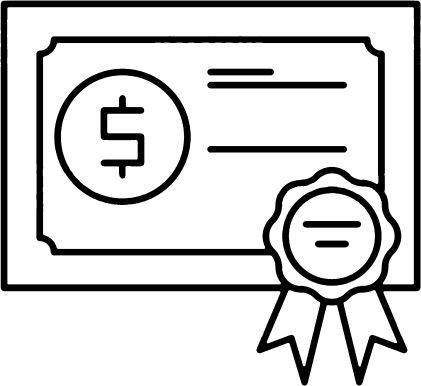
\includegraphics[width=0.75cm]{images/fond-share}};
					}
				
					\onslide<7>
					{
						\draw[thick,gray!50!white] (i) to [bend left=10] (s);
						\node at (0,1) {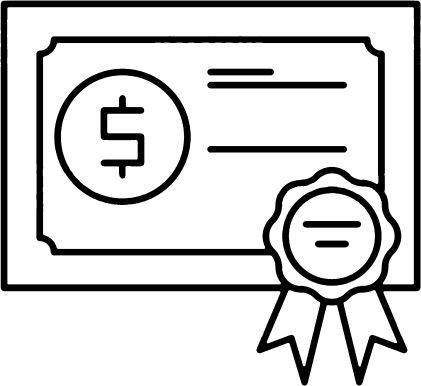
\includegraphics[width=0.75cm]{images/fond-share}};
					}
				\end{tikzpicture}
			\end{frame}
		
		\subsection{ETFs}
		\label{subsec:etfs}
		
		% \item Filterung: ESG, SRI, low carbon, controversial weapons (cw)
			\begin{frame}
				ETFs = exchange traded fund (börsengehandelter Fonds)
				\begin{definition}
					Investmentfonds, die man an der Börse handeln kann.\citewiki[Börsengehandelter\_Fonds]{B\%C3\%B6rsengehandelter\_Fonds}
				\end{definition}
				Meist synonym für \textit{Indexfonds}:\pause
				\begin{definition}
					Indexfonds sind Investmentfonds, deren Zusammensetzung sich möglichst exakt an der eines Index orientiert.\citewiki{Indexfonds}
				\end{definition}
				Orientieren = Nachbilden = Abbilden = Replikation
			\end{frame}
		
			\begin{frame}{Indexfonds}
				\begin{itemize}
					\item Bildet Index ab
					\item Passiver Fond
					\item Auswahl Aktien wie im Index
				\end{itemize}\vspace{0.25cm}
				\textbf{Beispiel DAX:}\vspace{0.25cm}
				\begin{tabularx}{\linewidth}{X|p{3cm}|X|X}
					Unternehmen & DAX-Gewichtung & iShares\footnote{\href{https://de.extraetf.com/etf-profile/DE0005933931?tab=components}{iShares Core DAX UCITS ETF (ISIN: DE0005933931)}} & Xtrackers\footnote{\href{https://de.extraetf.com/etf-profile/LU0274211480?tab=components}{Xtrackers DAX UCITS ETF (ISIN: LU0274211480)}}\\
					\hline
					Linde PLC & 10,10\% & 10,82\% & 10,89\% \\
					SAP & 8,50\% & 7,88\% & 7,86\%\\
					Siemens & 8,30\% & 7,37\% & 7,41\%
				\end{tabularx}
			\end{frame}
		
			\begin{frame}{Indexfonds}
				\begin{center}
					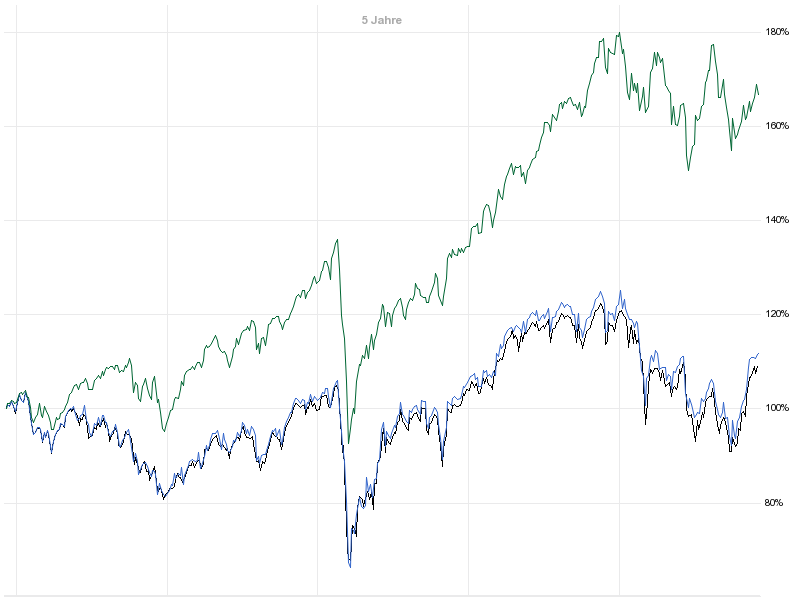
\includegraphics[height=0.75\textheight,trim=0 0 0 0.5cm]{images/dax-etf-benchmark}\footnote{Stand 04.12.2022; Quelle: \href{https://charts.comdirect.de/charts/benchmark_underlying.chart?HEIGHT=600&WIDTH=800&ID_BENCH1=20735&ID_BENCH2=12221463&ID_NOTATION=17138767&TIME_SPAN=5Y}{comdirect} / Grün: MSCI World; Schwarz: \href{https://www.comdirect.de/inf/etfs/LU0252633754}{Lyxor DAX UCITS ETF EUR ACC}; Blau: Dax Index}\\
				\end{center}
			\end{frame}
		
		\subsection{Derivate}
		
			\begin{frame}
				\begin{definition}
					Von normalen Finanzprodukten abgeleitetes Finanzprodukt mit fester Laufzeit.\citewiki{Derivat (Wirtschaft)}
				\end{definition}
				\textbf{Arten:}
				\begin{description}
					\item[Swaps] Tausch von Basiswerten (z.B. Zinsen) zur Absicherung.
					\item[Futures] Recht \& Pflicht auf festen Preis in der Zukunft.
					\item[Optionen] Future aber ohne Pflicht (\textrightarrow\ höhere Gebühren).
					\item[Forwards] Quasi Futures aber außerbörslich.
					\item[Zertifikat] Ähnlich zu Futures \& Optionen, aber in weird
				\end{description}
			\end{frame}
		
		\subsection{Konservative Finanzprodukte}
		
			\begin{frame}
				\begin{description}
					\item[Kopfkissen] Kein (negativ) Zins, keine Kosten, volle Inflation, keine Absicherung\pause
					\item[Girokonto] Keine Zinsen, Gebühren, Einlagensicherung\pause
					\item[Tagesgeld] Geringe Zinsen, keine Gebühren, Einlagensicherung, Überweisung nur von/an Referenzkonto\pause
					\item[Festgeld] Mäßige Zinsen, keine Gebühren, Einlagensicherung, feste Laufzeit\pause
					\item[Sparbuch] Kaum/keine Zinsen, keine Gebühren, Einlagensicherung, begrenztes abheben, lange Kündigungsfristen\pause
					\item[Lebensversicherung] Kaum Zinsen, Gebühren, Einlagensicherung\pause
					\item[Rohstoffe (z.B. Gold)] Recht volatil, Gewinn nur über Kurs, ethisch tlw. fragwürdig
				\end{description}
			\end{frame}
		
		\subsection{Kryptowährung}
		
			\begin{frame}
				\begin{definition}
					Kryptowährung/Krypto/Coin sind digitale Vermögenswerte, die auch als Tauschmittel fungieren.\citewiki[Kryptowährung]{Kryptow\%C3\%A4hrung}
				\end{definition}
			
				\begin{itemize}
					\item Derzeit nicht reguliert
					\item Reines Spekulationsobjekt
					\item Ein Träumchen für Kriminelle (Steuerhinterziehung, illegale Geschäfte, Scam)
					\item Steuerlich: Uff
					\begin{itemize}
						\item Privates Veräußerungsgeschäft (\textrightarrow\ Einkommenssteuer)
						\item Bis 600€ steuerfrei
						\item Bis 1 Jahr Haltedauer steuerpflichtig
					\end{itemize}
				\end{itemize}
			\end{frame}
	
	\section{Handelsplätze}
	
		\begin{frame}
			\tableofcontents[currentsection,hideallsubsections]
		\end{frame}
	
		\subsection{Börse}
		
			\begin{frame}
				\begin{definition}
					Organisierter Markt für standardisierte Handelsobjekte.\citewiki[Börse]{B\%Crse}
				\end{definition}
				\begin{itemize}
					\item Typische Handelsobjekte: Aktien, Anleihen, Derivate, ...
					\item Führt Angebot und Nachfrage zusammen \textrightarrow\ Entstehung Börsenkurse
					\begin{itemize}
						\item Kurse von Börse zu Börse leicht unterschiedlich
					\end{itemize}
					\item Überwacht durch z.B. BaFin oder SEC (Securities and Exchange Commission)
				\end{itemize}
			\end{frame}
		
			\begin{frame}
				Verschiedene Arten:
				\begin{itemize}
					\item Warenbörse
					\item Terminbörse (\textrightarrow\ Derivate)
					\item Wertpapierbörse (\textrightarrow\ Aktien, Anleihen)
					\item Energiebörse
					\item Emissionsrechtehandelssystem
				\end{itemize}
			\end{frame}
		
			\begin{frame}
				\centering
				\hspace{-0.5cm}
				\begin{tikzpicture}[->,>=stealth']
					\node (s) at (0,0) {
\includegraphics[width=0.75cm,trim=0 0 0 -1.35cm]{images/stonks-guy}};
					
					\node (i) at (2.5,-2) {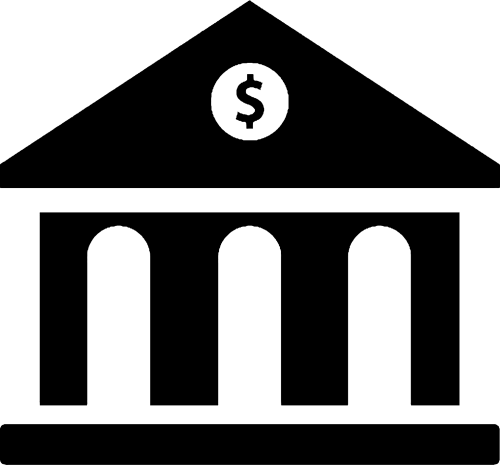
\includegraphics[width=0.75cm]{images/bank}};
					\node[below=-0.1cm of i, font=\scriptsize, align=center] {Bank\\(Depot)};
					
					\node (b) at (5,-4) {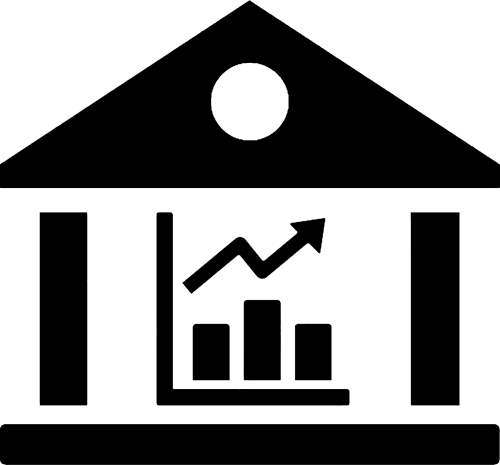
\includegraphics[width=0.75cm]{images/stockmarket}};
					\node[below=-0.1cm of b, font=\scriptsize] {Börse};
					
					\node (i2) at (7.5,-2) {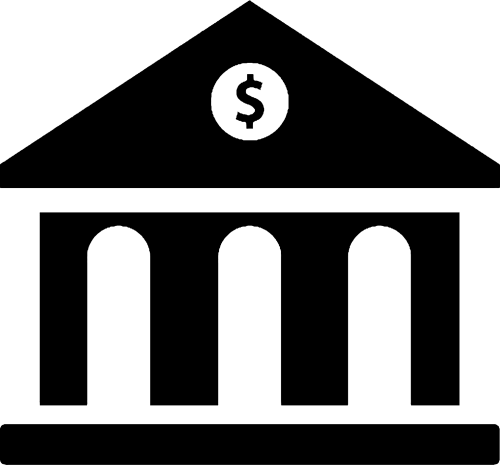
\includegraphics[width=0.75cm]{images/bank}};
					\node[below=-0.1cm of i2, font=\scriptsize, align=center] {Bank\\(Depot)};
					
					\node (s2) at (10,0) {\reflectbox{
\includegraphics[width=0.75cm,trim=0 0 0 -1.35cm]{images/stonks-guy}}};
					
					\onslide<1> {
						\draw (s) to [bend left=10] node[above right, align=center, font=\scriptsize] {Kauf-\\order} (i);
%						\smallmoney{(1.3, -0.5)}
%						\smallmoney{(1.375, -0.55)}
%						\smallmoney{(1.45, -0.6)}
%						\smallmoney{(1.525, -0.65)}
%						\smallmoney{(1.6, -0.7)}
					}
				
					\onslide<2-> {
						\draw[gray!50!white] (s) to [bend left=10] (i);
					}
					\onslide<2> {
%						\smallmoney{(2.5, -1.35)}
						
						\draw (i) to [bend left=10] node[above right, align=center, font=\scriptsize] {Kauf-\\order} (b);
%						\smallmoney{(3.875, -2.55)}
%						\smallmoney{(3.95, -2.6)}
%						\smallmoney{(4.025, -2.65)}
%						\smallmoney{(4.1, -2.7)}
					}
				
					\onslide<3-> {
						\draw[gray!50!white] (s) to [bend left=10] (i);
						\draw[gray!50!white] (i) to [bend left=10] (b);
						\node[below left=0.75cm and 0cm of b, font=\scriptsize, anchor=east] {Kauforder};
					}
					\onslide<3> {
						\draw (s2) to [bend right=10] node[above left, align=center, font=\scriptsize] {Verkaufs-\\order} (i2);
					}
				
					\onslide<4-> {
						\draw[gray!50!white] (s) to [bend left=10] (i);
						\draw[gray!50!white] (i) to [bend left=10] (b);
						\draw[gray!50!white] (s2) to [bend right=10] (i2);
					}
					\onslide<4> {
						\draw (i2) to [bend right=10] node[above left, align=center, font=\scriptsize] {Verkaufs-\\order} (b);
					}
				
					\onslide<5-> {
						\draw[gray!50!white] (s) to [bend left=10] (i);
						\draw[gray!50!white] (i) to [bend left=10] (b);
						\draw[gray!50!white] (s2) to [bend right=10] (i2);
						\draw[gray!50!white] (i2) to [bend right=10] (b);
						\node[below right=0.75cm and 0cm of b, font=\scriptsize, anchor=west] {Verkaufsorder};
					}
					\onslide<1-5> {
						\node[below right=0.075cm and -2.675cm of b, font=\tiny] {Orderbuch:};
						\node[below right=0.48cm and -2.55cm of b, minimum width=4.5cm, minimum height=0.5cm, draw, black] {};
					}
				
					\onslide<6-> {
						\node[below right=0.075cm and -2.675cm of b, font=\tiny] {Orderbuch:};
						\node[below right=0.48cm and -2.55cm of b, minimum width=4.5cm, minimum height=0.5cm, draw, green!75!black] {};
						\coordinate[below=0.75cm of b] (bb);
						\draw[<->] (bb)++(-0.5,0) -- +(1,0);
					}
					\onslide<7> {
						\smallmoney{(5, -1.45)}
						\draw (i) to [bend right=-7] (i2);
						\node at (5, -2.6) {
\includegraphics[width=0.5cm]{images/stock}};
						\draw (i2) to [bend right=-7] (i);
					}
					\onslide<8> {
						\node at (0, 0.8) {
\includegraphics[width=0.5cm]{images/stock}};
						\smallmoney{(10, 0.8)}
					}
				\end{tikzpicture}
			\end{frame}
		
		\subsection{Crowd-Investing}
		
			\begin{frame}
				\begin{definition}
					Viele Anleger investieren über das Internet kleine Beträge in Unternehmen (meist  Start-ups).\citewiki{Crowdinvesting}
				\end{definition}
				\textbf{Einfach gesagt:}\\
				Wie Crowdfunding nur mit Rendite.\n
				\textbf{Aber:}
				\begin{itemize}
					\item Hohe Rendite \textrightarrow\ hohes Risiko!
					\item Kaum gesetzliche Grundlagen \textrightarrow\ "`grauer Kapitalmarkt"'
				\end{itemize}
			\end{frame}
	
	\section{Privater Handel}
	
		\begin{frame}
			\tableofcontents[currentsection,hideallsubsections]
		\end{frame}
	
		\subsection{Depot, Bank, Broker}
		
			\begin{frame}{Bank}
				Reguliertes Kreditinstitut mit folgenden Geschäftsfeldern:
				\begin{itemize}
					\item Einlagen-, Kredit- und meistens Wertpapiergeschäft
					\item Wertpapierverwahrung
					\item Depotgeschäft
				\end{itemize}
			\end{frame}
		
			\begin{frame}{Depot}
				Verwahrstelle von Wertpapieren (Konto).
				\begin{itemize}
					\item Ggf. Depotführungsgebühren
					\item Angeboten von: Banken, Fondsgesellschaften, Broker
				\end{itemize}
			\end{frame}
		
			\begin{frame}{Broker}
				Finanzdienstleister zum Handel mit Wertpapieren.
				\begin{itemize}
					\item Engl. für Börsenmakler
					\item Meist sind Banken auch Broker
					\item Fokus reiner Broker: spekulative Privatanleger
				\end{itemize}
			\end{frame}
		
		\subsection{Investieren: Best practices + Tipps}
		
			\begin{frame}
				\begin{description}[labelwidth=0cm]
					\item[Diversifikation] Streuung von Anlagen zur Risikominimierung
					\item[Strategie] Einen Plan konsequent verfolgen (z.B. Core-Satellite-Strategie) \textrightarrow\  "`hin und her macht Taschen leer"'
					\item[Geduld] Verkauf erst in mehreren Jahren, sonst wäre es Spekulation
					\item[Gebühren] Depot- \& Ordergebühren, TER, Börsenplatzentgelte, Ausgabeaufschlag
					\item[Nachdenken] Clickbaits, Werbung, "`Beratung"' und "`Gruppen"'\footnote{\href{https://www.youtube.com/watch?v=dM-8-KuKprA}{PORSCHE CAYMAN S JUNGS! JAWOLL, JAAA! GEIL MAN!}} warten an jeder Ecke
					\item[Bildung] Wissen ist Macht, eigene Entscheidungen treffen
				\end{description}
			\end{frame}
		
			\begin{frame}{Welche Aktie/ETF/... kaufen?}
				DAS beste Finanzprodukt gibt es nicht!\pause
				\begin{itemize}
					\item Anlageziel klären
					\begin{itemize}
						\item Geld "`parken"'?
						\item Vermögensaufbau?
						\item Rente aufbessern?
						\item Etwas bewirken? (\textrightarrow\ impact investing)
					\end{itemize}\pause
					\item Risikobereitschaft klären
					\begin{itemize}
						\item Wie viel Geld bin ich bereit zu verlieren?
						\item Was ist mein worst-case Szenario? (Totalverlust? Verlust von $x$ \% Einsatz? ...)
					\end{itemize}\pause
					\item Art des Handels
					\begin{itemize}
						\item Einmaliger Kauf
						\item Aktives handeln (\textrightarrow\ trading $\neq$ investing)
						\item kontinuierliches investieren (\textrightarrow\ Sparplan)
					\end{itemize}
				\end{itemize}
			\end{frame}
		
			\begin{frame}{Welche Aktie/ETF/... kaufen?}
				\begin{itemize}
					\item Selbsteinschätzung
					\begin{itemize}
						\item Womit kenne ich mich aus? (z.B. Anleihen)
						\item Wo sind meine Interessen? (z.B. trading)
						\item Was traue ich mir zu?
						\item Wo habe ich Wissenslücken?
					\end{itemize}\pause
					\item Welche Produkte kommen \textit{nicht} in Frage? \pause
					\item Möchte ich einen Anlageberater? \pause
				\end{itemize}\n
				\textbf{Danach} konkretes klären:\\
				Welche Bank? Welches Depot? Welches exakte Finanzprodukt? Welche genaue Strategie? ...\n
				\textrightarrow\ Artikel der BaFin bzgl. Geldanlage: \href{https://www.bafin.de/SharedDocs/Veroeffentlichungen/DE/Fachartikel/2015/fa_bj_1506_geldanlage.html}{bafin.de}
			\end{frame}
	
	\section{Steuern}
	
		\begin{frame}
			\tableofcontents[currentsection,hideallsubsections]
		\end{frame}
	
		\begin{frame}{Steuern}
			\begin{center}
				\vspace{-0.5cm}
				
\includegraphics[height=0.85\textheight]{images/taxes-peter-parker}
			\end{center}
		\end{frame}
	
		\begin{frame}{Steuern}
			\begin{description}[labelwidth=0cm, align=right]
				\item[Kapitalertragssteuer] 25\% auf Kapitalerträge (+Soli +Kirchensteuer)
				\item[Sparerpauschbetrag] Freibetrag von 801€ pro Person pro Jahr
				\item[Vorabpauschale] Wird ggf. bei Fonds (z.B. ETFs) fällig
			\end{description}
		\end{frame}
	
		\begin{frame}{Steuer: HowTo}
			\begin{itemize}
				\item Abgeltungssteuer = Kapitalertragssteuer \textrightarrow\ Quellensteuer
				\item Quelle = Bank\pause
				\item Bank hält Steuer direkt ein
				\begin{itemize}
					\item Freistellungsauftrag stellen
					\item Verluste werden "`gut geschrieben"'
				\end{itemize}\pause
				\item Steuererklärung ggf. trotzdem sinnvoll
				\begin{itemize}
					\item Kein/falscher Freistellungsauftrag
					\item Sonstige Kapitalerträge
					\item Kapitalerträge im Ausland
				\end{itemize}
			\end{itemize}
		\end{frame}
	
	{
		\setbeamertemplate{background canvas}{
\includegraphics[width=\paperwidth]{images/questions.png}}
		\begin{frame}[plain]
			\begin{center}
				\vspace{1.5cm}
				Fragen?
			\end{center}
		\end{frame}
		\setbeamertemplate{background canvas}{ }
	}
\end{document}













